\chapter{Analisis}
Pada bab ini akan dibahas mengenai algoritma yang dipilih untuk menyembunyikan \textit{secret message}. Untuk itu penjelasannya akan dibagi menjadi beberapa bagian. Bagian pertama akan menjelaskan tentang gambaran umum algoritma yang dipakai. Selanjutnya akan dijelaskan bagaimana pemenggalan kata akan dilakukan. Ada pula bagian kamus sinonim, penjelasan lebih lengkapnya terdapat pada Bab \ref{sec:gambaran_umum} dan Bab \ref{sec:kamus_sinonim}. Setelah penjelasan tentang kamus sinonim, akan dijelaskan juga mengenai \textit{stego-cover} seperti apa yang akan dipakai, serta bagaimana proses \textit{embedding} dan \textit{extracting information}.

\section{Gambaran Algoritma Umum}
\label{sec:gambaran_umum}
\textit{Stego-cover} yang akan digunakan berupa \textit{text file} yang tentu terdiri dari banyak kata. Algoritma yang dipilih akan memanfaatkan banyaknya suku kata dalam suatu kata. Notasi \textit{c}(\textit{w}) akan digunakan untuk merepresentasikan banyaknya suku kata dalam suatu kata, dimana suatu katanya adalah \textit{w}. Diketahui bahwa \textit{c}(\textit{w}) dapat bernilai ganjil atau genap. Dua kemungkinan tersebut identik dengan bilangan biner. Dengan demikian diputuskan bahwa \textit{c}(\textit{w}) yang bernilai genap akan merepresentasikan 0 dan \textit{c}(\textit{w}) bernilai ganjil merepresentasikan 1. Dapat ditarik kesimpulan berarti 1 kata dapat diubah menjadi 1 bit bilangan biner. Jika sebuah \textit{stego-cover} memiliki 700 kata, berarti \textit{stego-cover} tersebut memiliki kapasitas sebesar 700 bit.

Setelah menemukan cara mengubah \textit{stego-cover} menjadi bilangan biner, \textit{secret message} juga harus diubah menjadi bilangan biner. Diketahui bahwa setiap karakter yang ditampilkan pada layar komputer, memiliki kode ASCII yang unik. Kode ASCII merupakan representasi numerik dari karakter seperti 'a', '1', atau '@'. Kode ASCII merupakan representasi numerik, berarti kode ASCII dapat diubah lagi menjadi bilangan biner. Sebagai contoh, jika sebuah \textit{secret message} terdiri dari n karakter dan tiap karakter diubah menjadi 7 bit bilangan biner dengan memanfaatkan kode ASCII, maka dibutuhkan minimal 7*\textit{n} bit \textit{stego-cover} untuk dapat menyembunyikan \textit{secret message} tersebut. 

\textit{Stego-cover} dan \textit{secret message} kini dapat diubah menjadi deret bilangan biner, \textit{stego-cover} harus dapat diubah lagi sedemikian rupa agar 7*\textit{n} deret biner pertamanya identik dengan deret biner \textit{secret message}. Sehingga saat proses ekstraksi, deret biner dari \textit{stego-cover} dapat diubah lagi menjadi karakter yang sesuai dengan \textit{secret message}. Karena \textit{c}(\textit{w}) dalam \textit{stego-cover} dapat bernilai 0 atau 1, ada kemungkinan \textit{c}(\textit{w}) tidak sesuai dengan angka biner dari \textit{secret message} yang akan disembunyikan. Untuk mengatasi hal ini, kata dengan nilai \textit{c}(\textit{w}) yang tidak sesuai, akan diganti dengan sinonim yang memiliki \textit{c}(\textit{w}) yang sesuai.

Tentunya semua kata yang ada pada \textit{stego-cover} harus memiliki sinonim agar setiap kata dapat memiliki \textit{c}(\textit{w}) yang bernilai 0 atau 1. Tesaurus merupakan buku referensi berupa daftar kata dengan sinonimnya\footnote{http://kbbi.web.id/tesaurus}. Namun karena format tesaurus yang memiliki banyak pengelompokan kata, seperti kata "bobol" bisa berarti "ambrol"/"hancur", bisa juga berarti "buyar"/"tembus". Lalu dari kata "bobol" bisa jadi "membobol" yang juga bisa berarti "membobok", bisa juga berarti "mencuri". Karena format yang terlalu rumit untuk dapat dibaca secara otomatis oleh program, maka diputuskan untuk membuat kamus sinonim yang lebih ringkas. Untuk kamus pada skripsi ini, telah disiapkan kamus sinonim yang daftar sinonimnya sebagian besar diambil dari tesaurus. Kamus sinonim ini berisi pasangan kata dengan sinonimnya pada tiap barisnya. Karena kamus sinonim dibuat sendiri, maka daftar kata yang ada di dalamnya, masih terbatas, artinya jika pengguna menambahkan \textit{stego-cover} baru, pengguna juga harus melengkapi sinonim yang belum terdaftar pada kamus sinonim.

\subsection{Pemenggalan Kata Menjadi Suku Kata}
Seperti yang telah dijelaskan pada Bab \ref{sec:gambaran_umum} untuk menghitung \textit{c}(\textit{w}) dibutuhkan proses pemenggalan kata menjadi suku kata. Untuk proses pemenggalan kata, akan menggunakan skripsi Frisca Sumarlin 2010 yang berjudul Aplikasi Pendongeng\cite{Frisca:2014}. Untuk mengenali suku kata dalam bahasa Indonesia, akan digunakan tiga tahap DFSA. Setiap masukan dari DFSA merupakan hasil DFSA tahap sebelumnya. Seperti yang telah dijelaskan, FSA memiliki prinsip kerja membaca hanya satu arah dan tidak bisa membaca mundur masukannya. Sedangkan untuk mengenali suku kata, untuk beberapa kasus kata dibutuhkan kemampuan untuk membaca mundur masukannya. Sebagai contoh, pada kata "anda", huruf ketiga adalah huruf konsonan sehingga pemenggalan suku kata dapat dilakukan pada saat membaca huruf ketiga.

Pada tahap 1 ini memang beberapa kata belum sesuai dengan aturan penyukuan kata yang benar, karena itu akan dilakukan tiga tahapan. Untuk diagramnya dapat dilihat pada Gambar \ref{fig:1-DFSA-1}.


\begin{figure}[H]
	\centering
	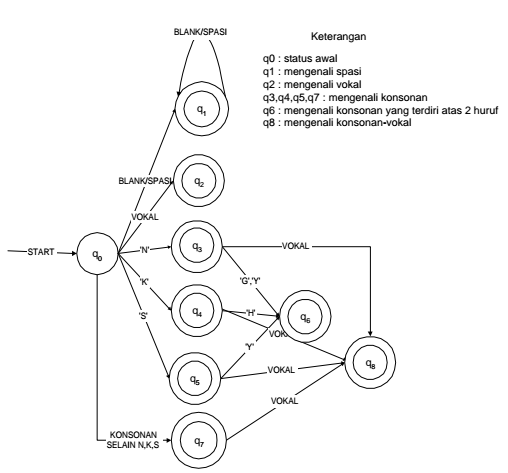
\includegraphics[scale=0.8]{Gambar/DFSA-1}
	\caption{Diagram Transisi DFSA tahap 1\cite{Thomas:2000}} 
	\label{fig:1-DFSA-1}
\end{figure}

Penjelasan tentang Diagram Transisi DFSA tahap 1 untuk mengenali spasi, vokal (V), konsonan yang terdiri dari 1 huruf (K), konsonan yang terdiri dari 2 huruf (KK), dan konsonan-vokal (KV) adalah sebagai berikut.

\begin{itemize}
	\item Perpindahan dari status awal (\textit{$q_0$}) ke \textit{$q_1$} adalah untuk mengenali spasi atau \textit{string} kosong.
	\item Perpindahan dari \textit{$q_0$} ke \textit{$q_2$} adalah untuk mengenali huruf vokal.
	\item Perpindahan dari \textit{$q_0$} ke \textit{$q_3$} adalah untuk mengenali huruf 'N'.
	\item Perpindahan dari \textit{$q_0$} ke \textit{$q_4$} adalah untuk mengenali huruf 'K'.
	\item Perpindahan dari \textit{$q_0$} ke \textit{$q_5$} adalah untuk mengenali huruf 'S'.
	\item Perpindahan dari \textit{$q_0$} ke \textit{$q_7$} adalah untuk mengenali huruf konsonan selain 'N', 'K', dan 'S'.
	\item Perpindahan dari \textit{$q_3$} ke \textit{$q_8$} adalah untuk mengenali pola suku kata VK.
	\item Perpindahan dari \textit{$q_3$} ke \textit{$q_6$} adalah untuk mengenali pola suku kata KK (ng dan ny).
	\item Perpindahan dari \textit{$q_3$} ke \textit{$q_8$} adalah untuk mengenali pola suku kata KV.
	\item Perpindahan dari \textit{$q_4$} ke \textit{$q_6$} adalah untuk mengenali pola suku kata KK (kh).
	\item Perpindahan dari \textit{$q_4$} ke \textit{$q_8$} adalah untuk mengenali pola suku kata KV.
	\item Perpindahan dari \textit{$q_5$} ke \textit{$q_6$} adalah untuk mengenali pola suku kata KK (sy).
	\item Perpindahan dari \textit{$q_5$} ke \textit{$q_8$} adalah untuk mengenali pola suku kata KV.
	\item Perpindahan dari \textit{$q_7$} ke \textit{$q_8$} adalah untuk mengenali pola suku kata KV.
\end{itemize}

Sebagai contoh, jika melakukan pemenggalan kata hanya dengan menggunakan DFSA tahap 1 saja, kata "gondok" tidak dapat dipotong secara sempurna. Berikut langkah-langkahnya.

\begin{itemize}
	\item Pada status awal (\textit{$q_0$}) huruf ke-1 'g' akan diperiksa.
	\item Pindah ke \textit{$q_7$} karena huruf 'g' merupakan huruf konsonan selain huruf 'N', 'K', dan 'S'.
	\item Huruf ke-2 'o' diperiksa dan pindah ke \textit{$q_8$} karena huruf 'o' merupakan huruf vokal. Suku kata ke-1 "go" disimpan, lanjut ke huruf selanjutnya dan mulai lagi dari \textit{$q_0$}.
	\item Huruf ke-3 'n' diperiksa dan pindah ke \textit{$q_3$} karena huruf ke-3 adalah huruf 'n'.
	\item Huruf ke-4 'd' diperiksa dan tidak memenuhi syarat untuk ke \textit{$q_8$} ataupun \textit{$q_6$}. Suku kata ke-2 "n" disimpan. Huruf ke-4 'd' kembali ke \textit{$q_0$}.
	\item Pindah ke \textit{$q_7$} karena huruf 'd' merupakan huruf konsonan selain huruf 'N', 'K', dan 'S'.
	\item Huruf ke-5 'o' diperiksa dan pindah ke \textit{$q_8$} karena '0' merupakan huruf vokal. Suku kata ke-3 "do" disimpan, lanjut ke huruf selanjutnya dan mulai lagi dari \textit{$q_0$}.
	\item Huruf ke-6 'k' diperiksa dan pindah ke \textit{$q_4$} karena huruf ke-6 adalah huruf 'K'. Suku kata ke-4 "k" disimpan. Tahap 1 selesai karena semua huruf telah melewati diagram transisi DFSA tahap 1.
	\item Didapatkan hasil pemenggalan suku kata "gondok" menjadi "go-n-do-k".
\end{itemize}

Dapat dilihat bahwa jika hanya menggunakan DFSA tahap 1, hasilnya masih belum sempurna. Pada tahap 1 hanya dikenali pola suku kata V, K, KV, dan KK. Selanjutnya, setelah melewati tahapan 1 DFSA, \textit{output}nya akan menjadi masukan untuk DFSA tahap 2. Pada tahap 2 ini harus dikenali V, KV, dan pengembangan dari ketiga pola yang dikenali pada tahap pertama. Pada tahap ini, pengembangan yang bisa dilakukan adalah V+K, K+KV, K+KV+K, K+K+KV, K+K+KV+K, K+KV+K, dan KV+K. Untuk digram transisi tahap kedua dapat dilihat pada Gambar \ref{fig:2-DFSA-2}.

\begin{figure}[H]
	\centering
	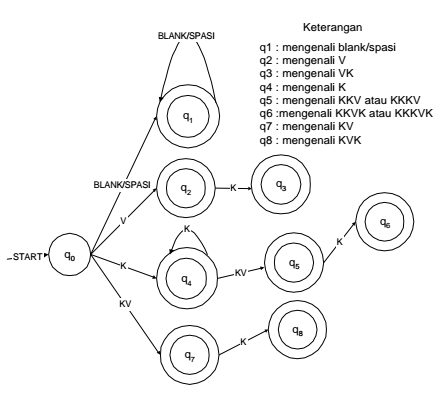
\includegraphics[scale=0.8]{Gambar/DFSA-2}
	\caption{Diagram Transisi DFSA tahap 2\cite{Thomas:2000} 
	\label{fig:2-DFSA-2}}
\end{figure}

Penjelasan tentang Diagram Transisi DFSA tahap 2 untuk mengenali pola suku kata V, VK, K, KKV, KKKV, KKVK, KKKVK, KV, dan KVK adalah sebagai berikut.

\begin{itemize}
	\item Perpindahan dari status awal (\textit{$q_0$}) ke \textit{$q_1$} adalah untuk mengenali spasi atau \textit{string} kosong.
	\item Perpindahan dari \textit{$q_0$} ke \textit{$q_2$} adalah untuk mengenali pola suku kata V.
	\item Perpindahan dari \textit{$q_0$} ke \textit{$q_4$} adalah untuk mengenali pola suku kata K.
	\item Perpindahan dari \textit{$q_0$} ke \textit{$q_7$} adalah untuk mengenali pola suku kata KV.
	\item Perpindahan dari \textit{$q_2$} ke \textit{$q_3$} adalah untuk mengenali pola suku kata VK.
	\item Perpindahan dari \textit{$q_4$} ke \textit{$q_4$} adalah untuk mengenali pola suku kata KK.
	\item Perpindahan dari \textit{$q_4$} ke \textit{$q_5$} adalah untuk mengenali pola suku kata KKV atau KKKV.
	\item Perpindahan dari \textit{$q_5$} ke \textit{$q_6$} adalah untuk mengenali pola suku kata KKVK atau KKKVK.
	\item Perpindahan dari \textit{$q_7$} ke \textit{$q_8$} adalah untuk mengenali pola suku kata KVK.
\end{itemize}

Pada tahap 2, masih ada tiga pola suku kata yang belum dapat dikenali, yaitu VKK, KVKK, dan KKVKK. Untuk itu masih dibutuhkan satu tahapan lagi untuk dapat mengenali pola-pola tersebut dan mengenali huruf diftong. Pada tahap ini hasil dari DFSA tahap kedua akan menjadi masukan bagi DFSA tahap terakhir yaitu tahap 3.

\begin{figure}[H]
	\centering
	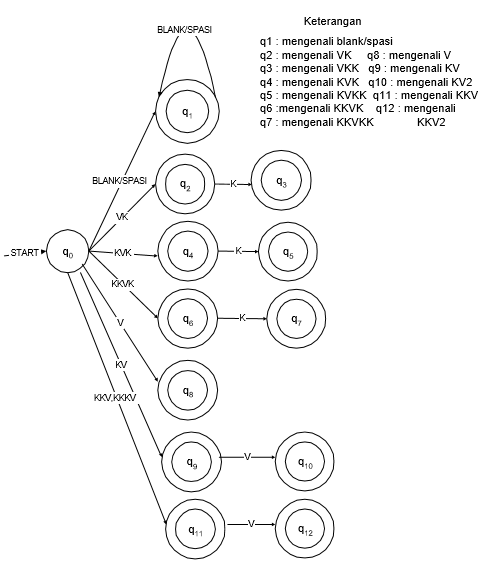
\includegraphics[scale=1]{Gambar/DFSA-3}
	\caption{Diagram Transisi DFSA tahap 3\cite{Thomas:2000}} 
	\label{fig:3-DFSA-3}
\end{figure}

Penjelasan tentang Diagram Transisi DFSA tahap 3 untuk mengenali pola suku kata VK, V, VKK, KV, KVK, KVV, KVKK, KKV, KKVK, KKVKK, dan KKVV adalah sebagai berikut.

\begin{itemize}
	\item Perpindahan dari status awal (\textit{$q_0$}) ke \textit{$q_1$} adalah untuk mengenali spasi atau \textit{string} kosong.
	\item Perpindahan dari \textit{$q_0$} ke \textit{$q_2$} adalah untuk mengenali pola suku kata VK.
	\item Perpindahan dari \textit{$q_0$} ke \textit{$q_4$} adalah untuk mengenali pola suku kata KVK.
	\item Perpindahan dari \textit{$q_0$} ke \textit{$q_6$} adalah untuk mengenali pola suku kata KKVK.
	\item Perpindahan dari \textit{$q_0$} ke \textit{$q_8$} adalah untuk mengenali pola suku kata V.
	\item Perpindahan dari \textit{$q_0$} ke \textit{$q_9$} adalah untuk mengenali pola suku kata KV.
	\item Perpindahan dari \textit{$q_0$} ke \textit{$q_{11}$} adalah untuk mengenali pola suku kata KKV atau KKKV.
	\item Perpindahan dari \textit{$q_2$} ke \textit{$q_3$} adalah untuk mengenali pola suku kata VKK.
	\item Perpindahan dari \textit{$q_4$} ke \textit{$q_5$} adalah untuk mengenali pola suku kata KVKK.
	\item Perpindahan dari \textit{$q_6$} ke \textit{$q_7$} adalah untuk mengenali pola suku kata KKVKK.
	\item Perpindahan dari \textit{$q_9$} ke \textit{$q_{10}$} adalah untuk mengenali pola suku kata KVV.
	\item Perpindahan dari \textit{$q_{11}$} ke \textit{$q_{12}$} adalah untuk mengenali pola suku kata KKVV atau KKKVV.
\end{itemize}

Untuk dapat membagi suku kata, diperlukan automata yang dapat menerima masukan berupa kata dan keluaran berupa suku kata. \textit{Finite State Transducer} merupakan \textit{finite state machine} yang memiliki dua pita, yaitu pita masukan dan pita keluaran. Automata yang telah dirancang adalah DFSA, di mana keluaran yang dihasilkan adalah dikenali atau tidak dikenali. Dengan merubah keluaran dari DFSA tersebut menjadi suku kata untuk setiap sekuens karakter yang telah dikenali, maka DFSA yang telah dirancang dapat dimanfaatkan untuk membagi kata menjadi suku kata. Atas dasar itu, DFSA dipilih untuk melakukan penyukuan kata.

Pemenggalan suku kata akan dipakai untuk mendapatkan banyak suku kata kata-kata yang terdapat pada \textit{stego-cover}, sehingga dapat dihitung banyak suku kata tiap katanya. Namun karena kumpulan \textit{stego-cover} yang akan dipakai dapat berupa cerita pendek(cerpen) atau puisi, maka isi dari \textit{stego-cover} tidak hanya berupa kata-kata alfabet saja, tetapi juga ada angka yang bisa berupa tanggal, kata serapan, dan lain-lain. Hal ini kemudian dapat menjadi hambatan, karena seperti yang kita ketahui bahwa angka tidak memiliki suku kata. Hambatan lainnya juga datang dari kata-kata dalam bahasa asing dan singkatan.

Setelah menemui hambatan-hambatan di atas, akhirnya diputuskan beberapa solusi. Pertama-tama, dari keseluruhan isi \textit{stego-cover}, tanda baca akan diabaikan (kecuali tanda penghubung '-'), sehingga yang akan dipenggal hanyalah kata-katanya saja. Satu digit angka akan dihitung sebagai satu suku kata, namun pada \textit{stego-cover} diputuskan untuk tidak boleh mengandung angka sama sekali, karena tidak memiliki sinonim. Semua singkatan atau kata dalam bahasa asing, akan dilakukan pemenggalan kata apa adanya.

\subsection{\textit{Stego-cover}}
\textit{Stego-cover} yang telah dikumpulkan berupa puisi dan cerpen. Alasan dipilihnya cerpen dan puisi sebagai \textit{stego-cover}, karena puisi umumnya menggunakan satu kata berulang-ulang, sehingga dapat mengurangi banyaknya kata yang disimpan pada kamus sinonim. Sedangkan cerpen yang dipilih memiliki jumlah kata yang cukup banyak, ini menandakan kapasitas penyimpanan yang cukup besar.

Dengan dipilihnya cerpen dan puisi sebagai \textit{stego-cover}, maka dibutuhkan skema komunikasi yang dapat menyamarkan artikel tersebut agar tidak menimbulkan kecurigaan oleh pihak lain. Skema komunikasi yang dipilih berupa komunikasi antara dua mahasiswa yang gemar mengirim puisi atau cerpen melalui \textit{email}. \textit{Email} yang dikirim mengandung \textit{stego-object} yang merupakan hasil dari \textit{embedding secret message} pada \textit{stego-cover}. Dengan skema komunikasi seperti ini, jika ada pihak lain yang membaca \textit{email} kedua mahasiswa tersebut, tidak akan mencurigai adanya kejanggalan karena kedua mahasiswa gemar berkirim puisi dan cerpen.

\subsection{Kamus sinonim}
\label{sec:kamus_sinonim}
Proses \textit{embedding} akan memanfaatkan daftar sinonim yang ada pada kamus sinonim. Kamus sinonim akan disimpan dalam sebuah \textit{file} dengan ekstensi .txt. Kamus sinonim dibuat dengan format seperti pada Gambar \ref{fig:6-format-kamus}. Kata pertama merupakan kata yang ada pada \textit{stego cover} dan kata di sebelahnya adalah sinonimnya. Format ini dipilih agar pencarian sinonim lebih mudah karena sudah berpasangan antara kata dan sinonimnya. Untuk skripsi ini telah disiapkan terlebih dahulu kamus sinonim yang dibuat secara manual. Pada kamus sinonim setiap kata yang ada pada \textit{stego-cover} memiliki sinonimnya sendiri. Referensi utama pembuatan kamus sinonim ini adalah tesaurus. Tesaurus merupakan buku referensi berupa daftar kata dengan sinonimnya\footnote{http://kbbi.web.id/tesaurus}. Kata-kata yang terdaftar di tesaurus adalah kata baku, sehingga jika pada \textit{stego-cover} terdapat kata yang tidak dapat ditemukan pada tesaurus, diperlukan penanganan tersendiri.

\begin{figure}[H]
	\centering
	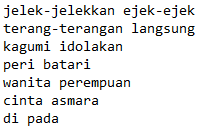
\includegraphics[scale=0.8]{Gambar/format-kamus}
	\caption{Format kamus sinonim} 
	\label{fig:6-format-kamus}
\end{figure}

Solusinya adalah dengan mengubah-ubah imbuhan pada awal atau akhir kalimat, namun tetap memperhatikan konteks kalimat tersebut. Sebagai contoh, pada \textit{stego-cover} terdapat kata 'menggendongnya', namun kata tersebut tidak dapat ditemukan pada tesaurus, karena terdapat imbuhan. Sehingga untuk sinonimnya dapat digunakan kata 'menggendong'. Kedua kata tersebut memiliki jumlah suku kata yang berbeda, namun memiliki arti yang sama.

Terdapat beberapa kata yang memang tidak memiliki sinonim dengan jumlah suku kata yang berbeda. Kata 'lama' memiliki 2 suku kata, sedangkan sinonim yang ada pada Tesaurus adalah 'lamban' dan 'lelet'. Kedua sinonimnya memiliki \textit{c}(\textit{w}) genap, tetapi yang dibutuhkan adalah \textit{c}(\textit{w}) ganjil. Hal ini dapat diatasi dengan menyamarkannya sebagai \textit{typo} atau kesalahan pengetikan. Contohnya dengan memasukkan kata 'lambaan' atau 'lamaa' sebagai sinonim dari kata 'lama'. Kata 'lambaan' dan 'lamaa', jika dipotong suku katanya dengan menggunakan pemotong suku kata yang telah dibuat, kedua kata tersebut memiliki \textit{c}(\textit{w}) ganjil.

\subsection{\textit{Embedding}}
Pada awal proses \textit{embedding} ada pemilihan \textit{stego-cover} yang akan dipakai untuk menyembunyikan pesan rahasia. Dari kumpulan \textit{stego-cover} akan diambil semua \textit{stego-cover} dengan kapasitas yang mencukupi untuk disisipkan \textit{secret message}. Dari banyak \textit{stego-cover} yang kapasitasnya mencukupi tersebut, dipilih satu secara acak untuk dijadikan masukan pada proses modifikasi \textit{stego-cover}.

Proses modifikasi akan memanfaatkan suku kata dan sinonim kata itu sendiri. Ide utamanya adalah dengan mengganti kata-kata tertentu yang ada dalam \textit{stego-cover} dengan kata-kata yang telah disediakan pada kamus sinonim, agar 7*\textit{n} deret bilangan biner pertama pada \textit{stego-cover} identik dengan deret bilangan biner \textit{secret message}. Kamus sinonim berisi semua kata yang ada pada \textit{stego cover} berpasangan dengan sinonimnya. Pasangan kata yang ada pada \textit{database} merupakan sinonim dengan \textit{c}(\textit{w}) yang berbeda (ganjil dan genap) dengan kata aslinya. \textit{Data Flow Diagram Embedding} dapat dilihat pada Gambar \ref{fig:4-dfd-embed}.

Penggantian kata pada \textit{stego-cover} ditentukan dari ASCII \textit{secret message} yang akan disembunyikan. ASCII (\textit{American Standard Code for Information Interchange}) merupakan format yang paling umum untuk \textit{file} teks yang ada di komputer dan internet\footnote{http://whatis.techtarget.com/definition/ASCII-American-Standard-Code-for-Information-Interchange}. Kode ASCII yang akan dipakai direpresentasikan dengan 7-bit angka biner, yang berarti ada 7 digit angka 0 atau 1. Pemilihan 7-bit ini dikarenakan kode ASCII yang umum dipakai hanya pada rentang desimal dari 0 sampai 127, sehingga jika menggunakan 8-bit, angka pertama(paling kiri) akan selalu bernilai 0. Dapat disimpulkan bahwa untuk menyisipkan 7-bit dibutuhkan 7 kata, 8-bit dibutuhkan 8 kata.  Untuk alasan memaksimalkan kapasitas penyisipan, maka diputuskan untuk merepresentasikan 1 karakter menjadi 7-bit.

\begin{figure}[H]
	\centering
	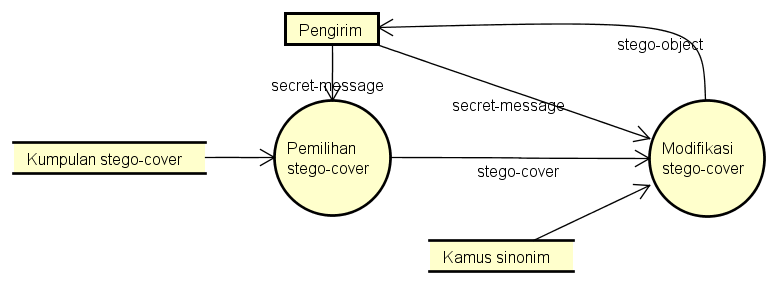
\includegraphics[scale=0.8]{Gambar/dfd-embed}
	\caption{\textit{Data Flow Diagram Embedding}} 
	\label{fig:4-dfd-embed}
\end{figure}

Setelah \textit{secret message} diubah menjadi deret bilangan biner dengan memanfaatkan kode ASCII, satu per satu digit kodenya akan dicocokkan dengan \textit{c}(\textit{w}) pada \textit{stego cover}. Kode digit pertama akan disisipkan pada kata pertama \textit{stego-cover}, digit kedua disisipkan pada kata kedua, dst. Jika \textit{c}(\textit{w}) pada \textit{stego-cover} tidak sesuai dengan digit kodenya, maka kata tersebut akan diganti dengan sinonimnya yang ada pada kamus sinonim. Pemberitahuan akan muncul jika ada kata yang sinonimnya tidak ditemukan pada kamus sinonim.

\subsubsection{Algoritma}
\label{algoritma}
Seperti yang telah dijelaskan sebelumnya, algoritma ini akan memanfaatkan kata yang ada pada \textit{stego-cover} untuk menyisipkan kode ASCII dari pesan rahasia ditambah kode ASCII karakter '\#' (untuk menandakan bahwa pesan rahasia telah berakhir). Proses penyisipan ini juga memanfaatkan kamus sinonim untuk mengubah kata asli yang ada pada \textit{stego-cover} dengan sinonim yang ada pada kamus sinonim jika \textit{c}(\textit{w}) tidak sesuai dengan kode ASCII pesan rahasia.

Algoritma \textit{embedding} pesan rahasia pada \textit{stego-cover} dengan memanfaatkan sinonim

\begin{enumerate}
	\item Meminta input berupa pesan rahasia(\textit{secret message}).
	\item Tiap karakter pada \textit{secret message} diubah menjadi kode ASCII 7-bit dan disimpan menjadi \textit{secret code}.
	\item Tambahkan deret biner 0100011, yang merupakan kode ASCII untuk karakter '\#' untuk menandakan bahwa \textit{secret message} telah berakhir.
	\item Jika n adalah banyak karakter yang ada pada \textit{secret message}, maka panjang \textit{secret code} = 7*(\textit{n}+1) (ditambah karakter '\#').
	\item Cari \textit{stego cover} yang dapat menampung \textit{secret code}. (Banyaknya kata yang ada dalam \textit{stego cover} $\geq$ panjang \textit{secret code}).
	\item Bangkitkan angka acak (r) dari \textit{range} 0 sampai banyaknya \textit{stego cover} yang dapat menampung \textit{secret code} - 1. 
	\item Buka \textit{file} ke-(r) dan baca per kata dengan mengabaikan tanda baca dan spasi.
	\item Untuk 7*(\textit{n}+1) kata pertama, lakukan pemenggalan kata dan dapatkan nilai \textit{c}(\textit{w}).
	\item Cocokkan nilai \textit{c}(\textit{w}) dengan angka ke-n yang ada pada \textit{secret code} secara berurutan. (\textit{c}(\textit{w}) kata ke-n dicocokkan dengan angka ke-n \textit{secret code}).
	\item Jika pada tahap 9 didapatkan \textit{c}(\textit{w}) yang tidak sesuai dengan angka ke-n \textit{secret code}, lanjut ke tahap 11. Jika sesuai, ulangi tahap 9.
	\item Cari sinonim kata tersebut pada kamus sinonim. Kata yang diambil hanya kata dengan nilai \textit{c}(\textit{w}) yang berbeda.
	\item Dari kata-kata yang didapatkan dari tahap 11, akan dilakukan pengambilan satu kata secara acak.
	\item Kata yang telah diambil dari tahap 12, akan menggantikan kata yang tidak sesuai sebelumnya.
	\item Kembali ke tahap 9.
\end{enumerate}

\subsection{\textit{Extracting Information}}
Pada proses pengekstraksian kembali pesan rahasia akan dibutuhkan input berupa \textit{stego-object} yang merupakan hasil dari \textit{embedding}. Perangkat lunak pertama-tama akan membaca secara keseluruhan inputnya, lalu melakukan pemenggalan kata sama seperti yang dilakukan pada saat proses \textit{embedding}. Selesai melakukan pemenggalan kata, dari tiap kata akan didapatkan $/sum$nya. Saat ini telah didapatkan deretan angka 0 dan 1 yang dinamakan \textit{secret code}. Saat proses \textit{embedding}, memang 1 karakter diubah menjadi kode ASCII 7-bit, namun \textit{java} menyediakan fungsi untuk mengubah deret biner 8-bit menjadi karakter. Sehingga untuk setiap 7-bit pada \textit{secret code} dapat ditambahkan angka 0 di paling kiri sebelum dijadikan \textit{input} pada fungsi \textit{java} tersebut.

Setelah selesai mengubah bit-bit yang ada menjadi karakter, hasilnya akan ditampilkan pada layar. Proses ektraksi ini melibatkan semua kata yang ada pada \textit{stego-object}, sehingga kata yang tidak disisipkan pesan rahasia pun ikut terekstraksi. Namun karena saat proses \textit{embedding} telah ditambahkan kode ASCII dari karakter '\#', maka \textit{secret message} berakhir saat ditemukan karakter '\#'. \textit{Data Flow Diagram Extract} dapat dilihat pada Gambar \ref{fig:5-dfd-extract}.

\begin{figure}[H]
	\centering
	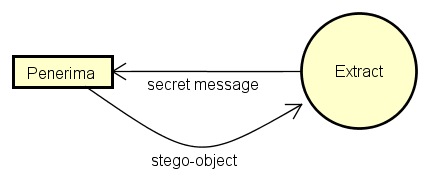
\includegraphics[scale=0.8]{Gambar/dfd-extract}
	\caption{\textit{Data Flow Diagram Extract}} 
	\label{fig:5-dfd-extract}
\end{figure}

\section{Analisis Use Case}

Diagram \textit{use case} perangkat lunak steganografi ini memiliki dua aktor, yaitu pengirim dan penerima. Pengirim berarti aktor yang akan melakukan \textit{embedding} dan mengirimkan \textit{stego-object}, sedangkan penerima berarti aktor yang menerima \textit{stego-object} dan melakukan \textit{extract information} untuk mendapatka \textit{secret message}. Diagram \textit{use case} dari perangkat lunak yang akan dibangun dapat dilihat pada Gambar \ref{fig:3_usecase}.

\begin{figure}[H]
	\centering
	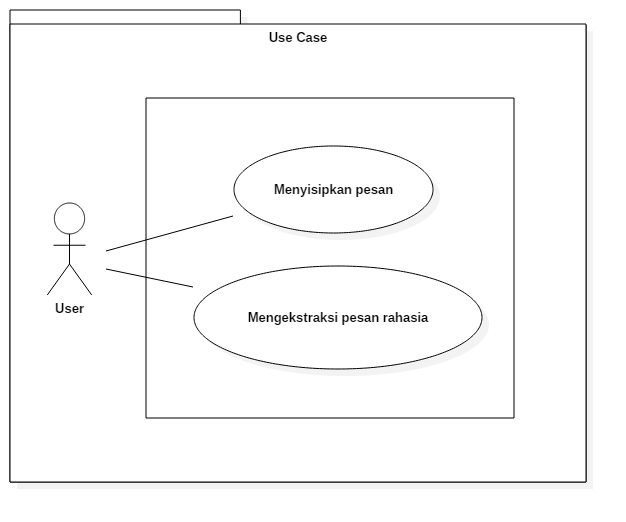
\includegraphics[scale=0.5]{Gambar/usecase}
	\caption{Use Case Diagram Perangkat Lunak Steganografi} 
	\label{fig:3_usecase}
\end{figure}

Dari diagram dapat dilihat enam \textit{use case}, yakni:
\begin{enumerate}
	\item \textbf{\textit{Embed}}, pengirim mengetikkan pesan rahasia yang akan disembunyikan.
	\item \textbf{Tambah \textit{stego-cover}}, pengirim menyalin teks sebagai \textit{stego-cover}. Jika pengirim menambahkan \textit{stego-cover}, maka pengirim wajib melengkapi sinonim yang belum terdaftar agar \textit{stego-cover} dapat digunakan.
	\item \textbf{Tambah sinonim}, pengirim mengetikkan kata beserta dengan sinonimnya pada masing-masing kotak yang telah disediakan.
	\item \textbf{Cek semua sinonim}, pengirim dapat memeriksa kata apa saja yang belum memiliki sinonim dengan menekan tombol yang telah disediakan.
	\item \textbf{\textit{Extract}}, penerima akan memasukkan \textit{stego-object} yang diterima.
	\item \textbf{Baca petunjuk}, pengirim dan penerima dapat membaca petunjuk terkait cara menggunakan perangkat lunak ini.
\end{enumerate}

\subsection{Skenario Use Case}

\begin{enumerate}
	\item \textbf{\textit{Embed}}
	\begin{itemize}
		\item Nama: \textit{Embed}
		\item Aktor: Pengirim
		\item Prakondisi: Pengirim mengetahui pesan rahasia yang akan disembunyikan
		\item Tujuan: Menghasilkan \textit{stego-object}.
		\item Skenario:
		\begin{table}[H]
		\centering
		\caption{Tabel Skenario \textit{Embed}}
		\begin{tabular}{| p{6.5cm} | p{6.5cm} |}\hline
		Pengirim & Sistem \\
		\hline
				1. Pengirim mengetikkan pesan rahasia yang akan disembunyikan. & \\
				\hline
				2. Pengirim menekan tombol \textit{Embed}. & 3. Sistem lalu akan mengubah pesan yang diketik menjadi kode ASCII. \\
				\hline
				& 4. Sistem mencari \textit{stego-cover} yang dapat menampung pesan yang sudah dalam bentuk ASCII. \\
				&	4.1. Tidak ada \textit{stego-cover} yang dapat menampung pesan.\\
				&	4.2. Sistem mengeluarkan peringatan bahwa pesan rahasia melebihi kapasitas dan kembali ke langkah 1.\\
				\hline
				& 5. Sistem melakukan proses \textit{embedding} dengan bantuan kamus sinonim. \\
				&	5.1. Proses \textit{embedding} gagal karena ada kata yang tidak ditemukan sinonimnya.\\
				&	5.2. Sistem mengembalikan daftar kata yang tidak terdaftar sinonimnya.\\
				&	5.3. Pengguna harus menambahkan sinonim kata yang belum terdaftar.\\
				\hline
				& 6. \textit{Stego-object} sebagai hasil dari proses \textit{embedding} akan ditampilkan pada kotak hasil.\\
		\hline
		\end{tabular}
		\end{table}
			
	\end{itemize}
	
	\item \textbf{Tambah \textit{stego-cover}}
	\begin{itemize}
		\item Nama: Tambah \textit{stego-cover}
		\item Aktor: Pengirim
		\item Prakondisi: Telah memiliki teks yang memenuhi syarat untuk dijadikan \textit{stego-cover}.
		\item Tujuan: Menambahkan variasi \textit{stego-cover}.
		\item Skenario:
		\begin{table}[H]
		\centering
		\caption{Tabel Skenario Tambah \textit{stego-cover}}
		\begin{tabular}{| p{6.5cm} | p{6.5cm} |}\hline
		Pengirim & Sistem \\
		\hline
				1. Pengirim mengetikkan judul untuk \textit{stego-cover} yang baru. & \\
				\hline
				2. Pengirim menyalin teks yang akan dijadikan \textit{stego-cover}. & \\
				\hline
				3. Pengirim menekan tombol Tambahkan Cover. & 4. Sistem akan membuat \textit{file} dengan nama \textit{file} sesuai dengan judul yang dimasukkan pengirim, dan menuliskan \textit{stego-cover} dalam \textit{file} tersebut. \\
				\hline
				& 5. Sistem menuliskan nama \textit{file} beserta kapasitas \textit{stego-cover} pada file lain yang merupakan daftar \textit{stego-cover} yang ada. \\
				\hline
				& 6. Akan tampil peringatan jika \textit{stego-cover} berhasil / gagal ditambahkan. \\
		\hline
		\end{tabular}
		\end{table}
	\end{itemize}
	
	\item \textbf{Tambah sinonim}
	\begin{itemize}
		\item Nama: Tambah sinonim
		\item Aktor: Pengirim
		\item Prakondisi: -
		\item Tujuan: Menambahkan daftar kata dan sinonimnya.
		\item Skenario:
		\begin{table}[H]
		\centering
		\caption{Tabel Skenario Tambah Sinonim}
		\begin{tabular}{| p{6.5cm} | p{6.5cm} |}\hline
		Pengirim & Sistem \\
		\hline
				1. Pengirim mengetikkan kata yang ada pada \textit{stego-cover}, yang akan ditambahkan sinonimnya. & \\
				\hline
				2. Pengirim mengetikkan sinonim dari kata pada tahap 1. & 3. Sistem akan menghitung nilai \textit{c}(\textit{w}) kata pada tahap 1 dan \textit{c}(\textit{w}) sinonim pada tahap 2. \\
				\hline
				& 4. Sistem akan menambahkan sinonim karena nilai \textit{c}(\textit{w}) pada tahap 1 berbeda dengan nilai \textit{c}(\textit{w}) pada tahap 2. \\
				& 4.1. Sistem tidak menambahkan sinonim karena nilai \textit{c}(\textit{w}) pada tahap 1 sama dengan nilai \textit{c}(\textit{w}) tahap 2. \\
				& 4.2. Sistem menampilkan hasil pemotongan kata dari sinonim. \\
				\hline
				& 5. Sistem menampilkan pesan bahwa sinonim berhasil ditambahkan. \\
				\hline
				& 6. Akan tampil peringatan jika \textit{stego-cover} berhasil / gagal ditambahkan. \\
		\hline
		\end{tabular}
		\end{table}
	\end{itemize}
	
	\item \textbf{Cek semua sinonim}
	\begin{itemize}
		\item Nama: Cek semua sinonim
		\item Aktor: Pengirim
		\item Prakondisi: -
		\item Tujuan: Menginformasikan kata mana saja yang belum memiliki sinonim.
		\item Skenario:
		\begin{table}[H]
		\centering
		\caption{Tabel Skenario Cek Semua Sinonim}
		\begin{tabular}{| p{6.5cm} | p{6.5cm} |}\hline
		Pengirim & Sistem \\
		\hline
				1. Pengirim menekan tombol Periksa semua sinonim. & 2. Sistem akan memeriksa semua kata yang ada pada semua \textit{stego-cover} untuk dicari sinonimnya pada kamus sinonim. \\
				\hline
				& 3. Kata yang belum memiliki sinonim akan ditampilkan oleh sistem. \\
				& 3.1. Pengirim harus menambahkan sinonim untuk kata yang ditampilkan.\\
		\hline
		\end{tabular}
		\end{table}
	\end{itemize}
	
	\item \textbf{\textit{Extract}}
	\begin{itemize}
		\item Nama: \textit{Extract}
		\item Aktor: Penerima
		\item Prakondisi: Telah memiliki \textit{stego-object} yang dihasilkan dari perangkat lunak yang sama.
		\item Tujuan: Mengkestraksi pesan rahasia dari \textit{stego-object}.
		\item Skenario:
		\begin{table}[H]
		\centering
		\caption{Tabel Skenario \textit{Extract}}
		\begin{tabular}{| p{6.5cm} | p{6.5cm} |}\hline
		Pengirim & Sistem \\
		\hline
				1. Penerima menyalin \textit{stego-object} yang didapat dari perangkat yang sama. & 2. Penerima menekan tombol \textit{Extract}. \\
				\hline
				& 3. Sistem akan mengeksekusi fungsi ekstraksi. \\
				\hline
				& 4. \textit{Secret message} yang merupakan hasil ekstraksi akan ditampilkan\\
				& 4.1. Sistem tidak menemukan karakter '\#', ditampilkan pesan error. \\
		\hline
		\end{tabular}
		\end{table}
	\end{itemize}
	
	\item \textbf{Baca petunjuk}
	\begin{itemize}
		\item Nama: Baca petunjuk
		\item Aktor: Pengirim atau penerima
		\item Prakondisi: -
		\item Tujuan: Memberi pemahaman kepada pengirim dan penerima mengenai cara menggunakan perangkat lunak ini.
		\item Skenario:
		\begin{table}[H]
		\centering
		\caption{Tabel Skenario Baca Petunjuk}
		\begin{tabular}{| p{6.5cm} | p{6.5cm} |}\hline
		Pengirim & Sistem \\
		\hline
				1. Pengirim atau penerima membaca petunjuk tentang \textit{embedding}. & \\
				\hline
				2. Pengirim atau penerima membaca petunjuk tentang \textit{extract}. & \\
				\hline
				3. Pengirim atau penerima membaca petunjuk tentang \textit{cover} (\textit{stego-cover}). & \\
				\hline
				4. Pengirim atau penerima membaca petunjuk tentang sinonim. & \\
		\hline
		\end{tabular}
		\end{table}
	\end{itemize}
\end{enumerate}

\subsection{Analisis Diagram Kelas}

Diagram kelas perangkat lunak steganografi dapat dilihat pada Gambar \ref{fig:3_classdiagram}

\begin{figure}[H]
	\centering
	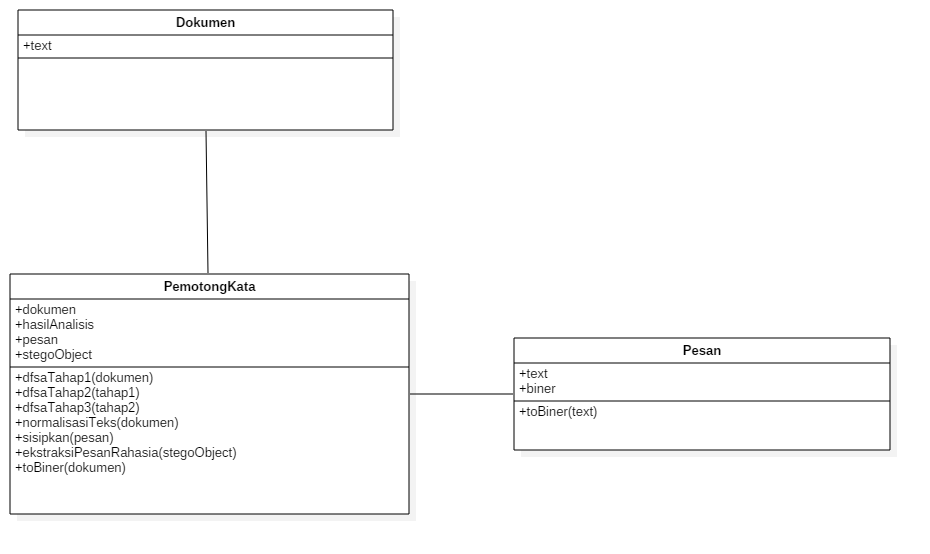
\includegraphics[scale=0.6]{Gambar/classdiagram}
	\caption{Class Diagram perangkat lunak steganografi} 
	\label{fig:3_classdiagram}
\end{figure}

Keterangan atas diagram kelas akan dijelaskan sebagai berikut:

\begin{enumerate}

	\item \textbf{Kelas \textit{Extractor}}
	\begin{itemize}
		\item Atribut pk, untuk melakukan pemenggalan kata.
		\item Fungsi ekstraksi, memiliki parameter stegoObject, untuk melakukan proses \textit{extract}.
	\end{itemize}

	\item \textbf{Kelas PemotongKata}
	\begin{itemize}
		\item Fungsi dfsaTahap1, memiliki parameter pesan, mengembalikan keluaran berupa hasil proses dfsa tahap pertama.
		\item Fungsi dfsaTahap2, memiliki parameter tahap1 yang merupakan keluaran dfsaTahap1 dan mengembalikan hasil proses dfsa tahap kedua.
		\item Fungsi dfsaTahap3, memiliki parameter tahap2 yang merupakan keluaran dfsaTahap2 dan mengembalikan hasil penyukuan kata akhir.
		\item normalisasiTeks, memiliki parameter dokumen. Parameter dokumen merupakan dokumen yang ingin dihilangkan semua tanda bacanya, sehingga siap untuk dilakukan pemenggalan kata.
		\item Fungsi toBiner, memiliki parameter dokumen. Parameter dokumen merupakan dokumen yang siap untuk dilakukan pemenggalan kata, sehingga fungsi ini akan melakukan pemenggalan kata dan didapatkan \textit{c}(\textit{w}) untuk semua kata yang ada dalam dokumen.
		\item Fungsi penggalKata, memiliki parameter pesan, melakukan pemenggalan kata dengan menggunakan fungsi dfsaTahap1, dfsaTahap2, dan dfsaTahap3.
	\end{itemize}

	\item \textbf{Kelas \textit{Embedder}}
	\begin{itemize}
		\item Atribut kamus, untuk mencari sinonim.
		\item Atribut pk, untuk melakukan pemenggalan kata.
		\item Atribut dok, untuk menyimpan kumpulan \textit{stego-cover}.
		\item Atribut hasilAnalisis, untuk menyimpan kumpulan \textit{c}(\textit{w}) dari dokumen.
		\item Fungsi sisipkan, memiliki parameter pesan, untuk melakukan proses \textit{embedding}.
	\end{itemize}

	\item \textbf{Kelas Dokumen}
	\begin{itemize}
		\item Atribut \textit{text}, untuk menampung teks dari dokumen berupa \textit{string}.
		\item \textit{Constructor} Dokumen, memiliki parameter bertipe \textit{string}, parameter akan mengisi atribut teks.
		\item Fungsi getText, merupakan \textit{getter} untuk atribut \textit{text}.
	\end{itemize}
	
	\item \textbf{Kelas KamusSinonim}
	\begin{itemize}
		\item Atribut fr, untuk membuka \textit{file}.
		\item Atribut br, untuk membaca file yang dibuka fr.
		\item Fungsi cariSinonim, memiliki parameter text, untuk mencari sinonim dari parameter.
		\item Fungsi tambahSinonim, memiliki parameter kata dan sinonim, untuk menambah sinonim baru.
	\end{itemize}
	
\end{enumerate}